\documentclass[border=14pt]{standalone}
\usepackage{tikz}
\usepackage{amsmath}
\usetikzlibrary{positioning,arrows.meta,fit,backgrounds,calc}
\begin{document}
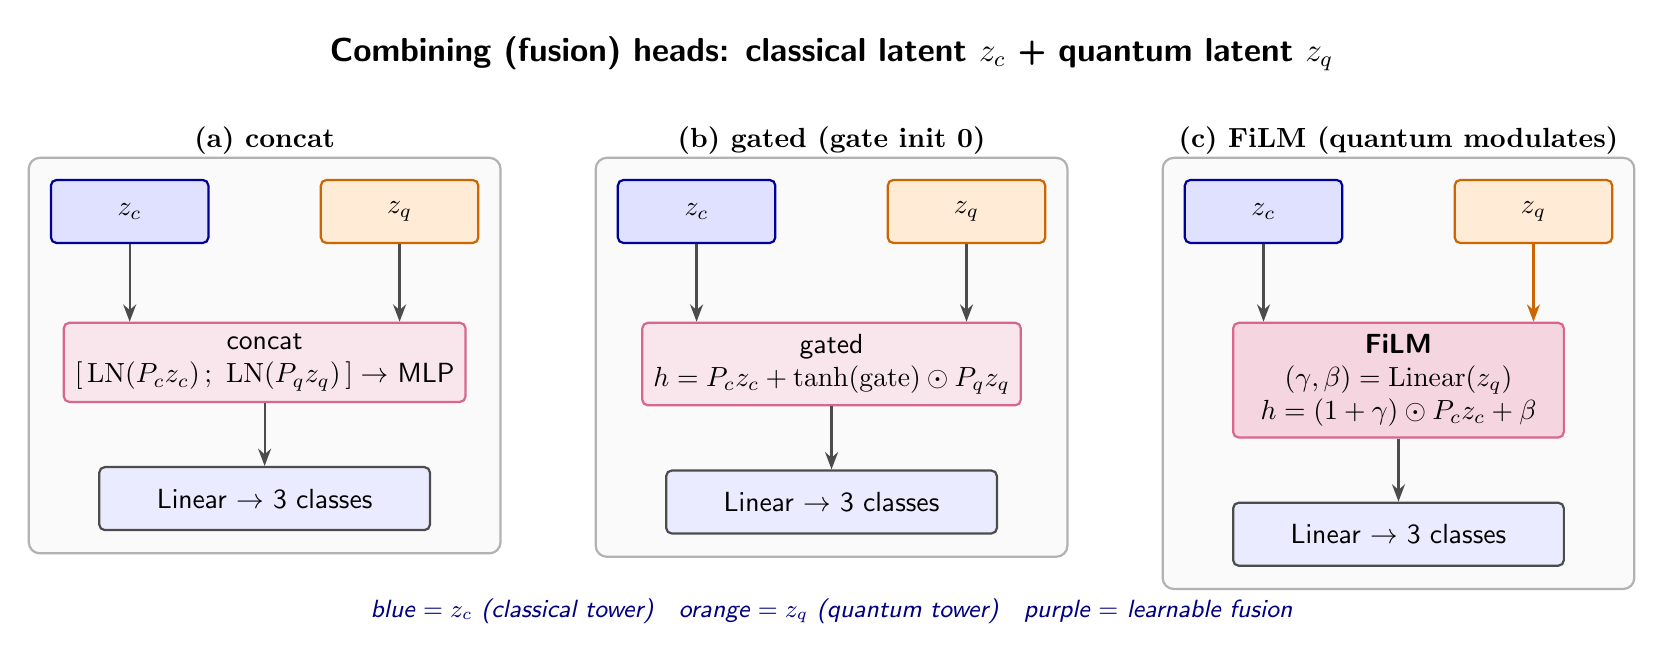
\begin{tikzpicture}[
  font=\sffamily,
  box/.style={rectangle,rounded corners=2pt,draw=black!70,thick,fill=blue!8,
              minimum height=8mm,minimum width=30mm,align=center,inner sep=4pt},
  cin/.style={box,fill=blue!12,draw=blue!60!black,minimum width=20mm},
  qin/.style={box,fill=orange!16,draw=orange!80!black,minimum width=20mm},
  fuse/.style={box,fill=purple!10,draw=purple!60,minimum width=42mm},
  panel/.style={rectangle,rounded corners=4pt,draw=black!30,thick,fill=black!2,inner sep=8pt},
  arr/.style={-{Stealth[length=2.2mm]},thick,black!70},
]
% ---------- Panel A: concat ----------
\begin{scope}[local bounding box=A]
  \node[cin] (ac) {$z_c$};
  \node[qin,right=14mm of ac] (aq) {$z_q$};
  \node[fuse,below=14mm of $(ac)!0.5!(aq)$] (af)
     {concat\\$[\,\mathrm{LN}(P_c z_c)\,;\ \mathrm{LN}(P_q z_q)\,]\to$ MLP};
  \node[box,below=8mm of af,minimum width=42mm] (ah) {Linear $\to$ 3 classes};
  \draw[arr] (ac.south) -- (ac.south|-af.north);
  \draw[arr] (aq.south) -- (aq.south|-af.north);
  \draw[arr] (af)--(ah);
\end{scope}
\node[font=\bfseries,above=2mm of A.north] {(a) concat};
\begin{scope}[on background layer]\node[panel,fit=(A)(af)(ah)] {};\end{scope}

% ---------- Panel B: gated ----------
\begin{scope}[local bounding box=B,shift={(72mm,0)}]
  \node[cin] (bc) {$z_c$};
  \node[qin,right=14mm of bc] (bq) {$z_q$};
  \node[fuse,below=14mm of $(bc)!0.5!(bq)$] (bf)
     {gated\\$h=P_c z_c+\tanh(\mathrm{gate})\odot P_q z_q$};
  \node[box,below=8mm of bf,minimum width=42mm] (bh) {Linear $\to$ 3 classes};
  \draw[arr] (bc.south) -- (bc.south|-bf.north);
  \draw[arr] (bq.south) -- (bq.south|-bf.north);
  \draw[arr] (bf)--(bh);
\end{scope}
\node[font=\bfseries,above=2mm of B.north] {(b) gated (gate init 0)};
\begin{scope}[on background layer]\node[panel,fit=(B)(bf)(bh)] {};\end{scope}

% ---------- Panel C: FiLM ----------
\begin{scope}[local bounding box=C,shift={(144mm,0)}]
  \node[cin] (cc) {$z_c$};
  \node[qin,right=14mm of cc] (cq) {$z_q$};
  \node[fuse,below=14mm of $(cc)!0.5!(cq)$,fill=purple!16] (cf)
     {\textbf{FiLM}\\$(\gamma,\beta)=\mathrm{Linear}(z_q)$\\$h=(1+\gamma)\odot P_c z_c+\beta$};
  \node[box,below=8mm of cf,minimum width=42mm] (ch) {Linear $\to$ 3 classes};
  \draw[arr] (cc.south) -- (cc.south|-cf.north);
  \draw[arr,orange!80!black] (cq.south) -- (cq.south|-cf.north);
  \draw[arr] (cf)--(ch);
\end{scope}
\node[font=\bfseries,above=2mm of C.north] {(c) FiLM (quantum modulates)};
\begin{scope}[on background layer]\node[panel,fit=(C)(cf)(ch)] {};\end{scope}

\node[font=\sffamily\large\bfseries] at ($(A.north)!0.5!(C.north)+(0,16mm)$)
  {Combining (fusion) heads: classical latent $z_c$ + quantum latent $z_q$};
\node[font=\sffamily\small\itshape,text=blue!50!black] (cleg)
  at ($(A.south)!0.5!(C.south)+(0,-8mm)$)
  {blue $=z_c$ (classical tower)\quad orange $=z_q$ (quantum tower)\quad
   purple $=$ learnable fusion};
\end{tikzpicture}
\end{document}
